\documentclass{article}
\usepackage[paperwidth=21cm,paperheight=15cm,margin=0.3cm]{geometry}
\usepackage{tikz}
\usepackage{amsmath}
\pagestyle{empty}
\begin{document}
\centering
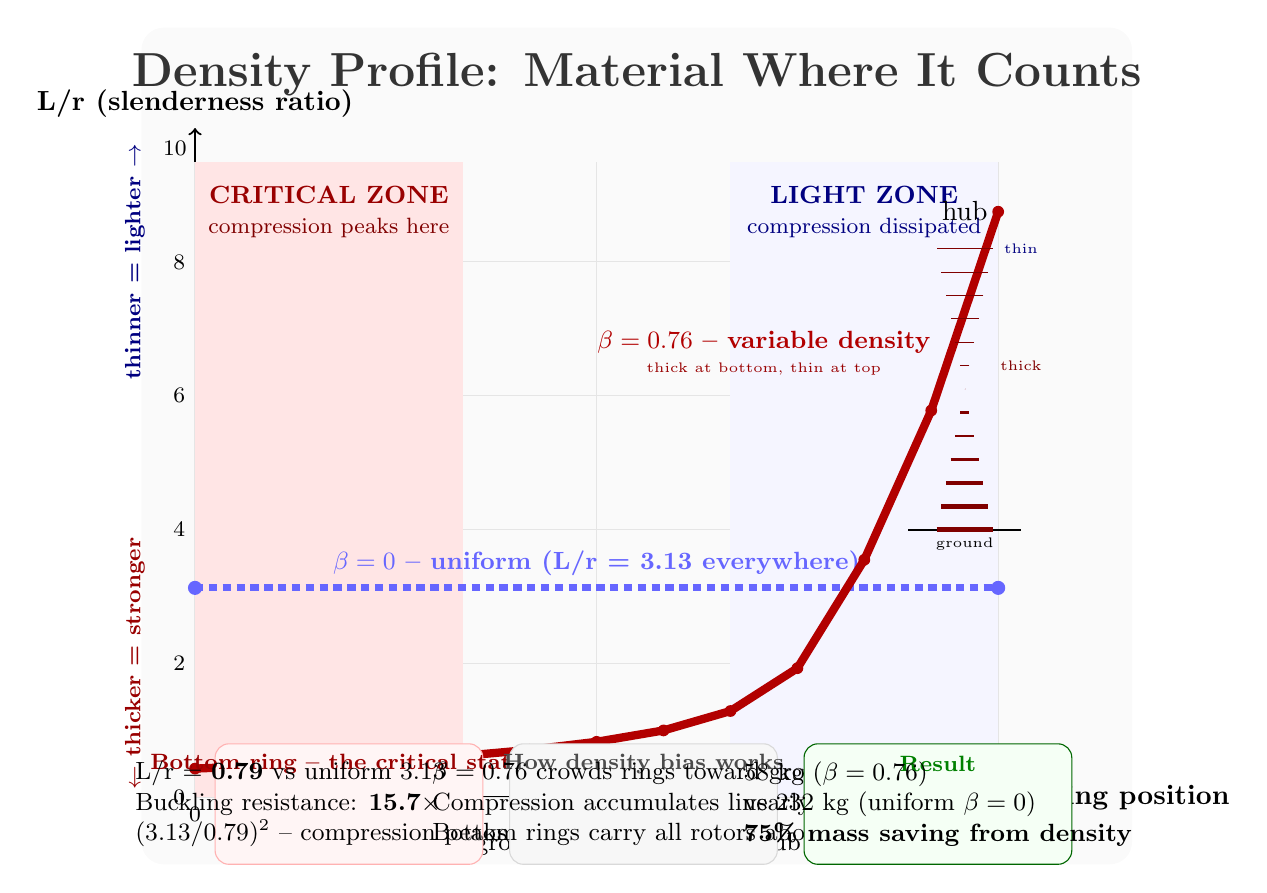
\begin{tikzpicture}[scale=0.85]

% Background
\fill[black!2, rounded corners=8pt] (-0.8,-1.0) rectangle (14.0,11.5);
\node[font=\bfseries\LARGE, black!80] at (6.6,10.8) {Density Profile: Material Where It Counts};

% === AXES ===
\draw[->, thick] (0,0) -- (0,10.0) node[above, font=\bfseries] {L/r (slenderness ratio)};
\node[font=\footnotesize\bfseries, rotate=90, red!60!black] at (-0.9,2.0) {$\leftarrow$ thicker = stronger};
\node[font=\footnotesize\bfseries, rotate=90, blue!50!black] at (-0.9,8.0) {thinner = lighter $\rightarrow$};

\draw[->, thick] (0,0) -- (12.5,0) node[right, font=\bfseries] {Ring position};
\node[font=\small] at (6.25,-0.7) {0 = ground \hspace{1.5cm} 1.0 = hub};

\foreach \x in {0,2,4,6,8,10,12} {\draw[gray!20] (\x,0) -- (\x,9.5);}
\foreach \y in {0,2,4,6,8} {\draw[gray!20] (0,\y) -- (12,\y);}
\foreach \y in {0,2,4,6,8} {\node[left, font=\footnotesize] at (0,\y) {\y};}
\node[font=\footnotesize] at (-0.3,9.7) {10};
\node[font=\footnotesize] at (0,-0.25) {0};
\node[font=\footnotesize] at (12,-0.25) {1.0};

% === COMPRESSION ZONE SHADING ===
\fill[red!10] (0,0) rectangle (4,9.5);
\node[font=\bfseries\small, red!60!black] at (2.0,9.0) {CRITICAL ZONE};
\node[font=\footnotesize, red!50!black] at (2.0,8.5) {compression peaks here};

\fill[blue!4] (8,0) rectangle (12,9.5);
\node[font=\bfseries\small, blue!50!black] at (10.0,9.0) {LIGHT ZONE};
\node[font=\footnotesize, blue!50!black] at (10.0,8.5) {compression dissipated};

% === UNIFORM (\beta=0) ===
\draw[blue!60, line width=2.5pt, densely dashed] (0,3.13) -- (12,3.13);
\fill[blue!60] (0,3.13) circle (3pt);
\fill[blue!60] (12,3.13) circle (3pt);
\node[blue!60, font=\bfseries\small] at (6.0,3.5) {$\beta=0$ -- uniform (L/r = 3.13 everywhere)};

% === VARIABLE DENSITY (\beta=0.76) ===
\draw[red!70!black, line width=3.0pt]
    (0,0.43) -- (1,0.47) -- (2,0.51) -- (3,0.56) -- (4,0.62)
    -- (5,0.71) -- (6,0.83) -- (7,1.00) -- (8,1.29) -- (9,1.93)
    -- (10,3.55) -- (11,5.78) -- (12,8.75);
\foreach \i/\y in {0/0.43,1/0.47,2/0.51,3/0.56,4/0.62,5/0.71,6/0.83,7/1.00,8/1.29,9/1.93,10/3.55,11/5.78,12/8.75} {
    \fill[red!70!black] (\i,\y) circle (2.5pt);
}
\node[red!70!black, font=\bfseries\small] at (8.5,6.8) {$\beta=0.76$ -- variable density};
\node[font=\tiny, red!60!black] at (8.5,6.4) {thick at bottom, thin at top};

% === INSET: TAPERED RING STACK (right side) ===
\begin{scope}[xshift=11.5cm, yshift=4.0cm, scale=0.7]
  \draw[thick] (-1.2,0) -- (1.2,0);
  \node[font=\tiny] at (0,-0.3) {ground};
  \foreach \i/\w in {0/2.0,1/1.7,2/1.4,3/1.15,4/0.95,5/0.78,6/0.65,7/0.55,8/0.45,9/0.38,10/0.32,11/0.28,12/0.25} {
  \draw[red!50!black, line width=\w pt] ({-0.6+0.1*\i},\i*0.5) -- ({0.6-0.1*\i},\i*0.5);
  }
  \node[font=\tiny, red!50!black] at (1.2,3.5) {thick};
  \node[font=\tiny, blue!50!black] at (1.2,6.0) {thin};
  \node at (0,6.8) {hub};
\end{scope}

% === COMPARTMENTALIZED INFO PANELS (bottom strip) ===
% Panel A -- The critical station
\fill[red!4, draw=red!30, rounded corners=5pt] (0.3,-1.0) rectangle (4.3,0.8);
\node[font=\bfseries\footnotesize, red!60!black] at (2.3,0.5) {Bottom ring -- the critical station};
\node[font=\small, align=left] at (2.3,-0.1) {
  L/r = \textbf{0.79} vs uniform 3.13\\
  Buckling resistance: \textbf{15.7$\times$}\\
  $(3.13/0.79)^2$ -- compression peaks here
};

% Panel B -- The mechanism
\fill[black!3, draw=gray!30, rounded corners=5pt] (4.7,-1.0) rectangle (8.7,0.8);
\node[font=\bfseries\footnotesize, black!70] at (6.7,0.5) {How density bias works};
\node[font=\small, align=left] at (6.7,-0.1) {
  $\beta=0.76$ crowds rings toward ground.\\
  Compression accumulates linearly.\\
  Bottom rings carry all rotors above.
};

% Panel C -- The result
\fill[green!4, draw=green!40!black, rounded corners=5pt] (9.1,-1.0) rectangle (13.1,0.8);
\node[font=\bfseries\footnotesize, green!50!black] at (11.1,0.5) {Result};
\node[font=\small, align=left] at (11.1,-0.1) {
  58 kg $(\beta=0.76)$\\
  vs 232 kg (uniform $\beta=0$)\\
  \textbf{75\% mass saving from density}
};

\end{tikzpicture}
\end{document}
